\documentclass[12pt, a4paper, twoside]{article}
\usepackage[utf8]{inputenc}
\usepackage{graphicx}
\graphicspath{ {images/} }
\PassOptionsToPackage{hyphens}{url}
\usepackage{hyperref}
\usepackage{rotating}
\usepackage{pdflscape}

\title{CalculiX Benchmark Study:\\Rotating Hollow Disk}
\author{Süleyman Muti}
\date{May 19, 2020}

\begin{document}


\maketitle


\begin{abstract}
	
Theoretical and finite element analysis results of the rotating hollow disk problem are compared. The free and open-source finite element analysis software CalculiX is used. The hollow disk is modelled using axisymmetric elements.

\end{abstract}


\section{Theory of Elasticity: Thin Rotating\\Hollow Disk}
Rotating hollow disk problem is shown in Figure ~\ref{fig:rotating_disk_axisymmetric}. 

\begin{figure}[h]
	\centering
	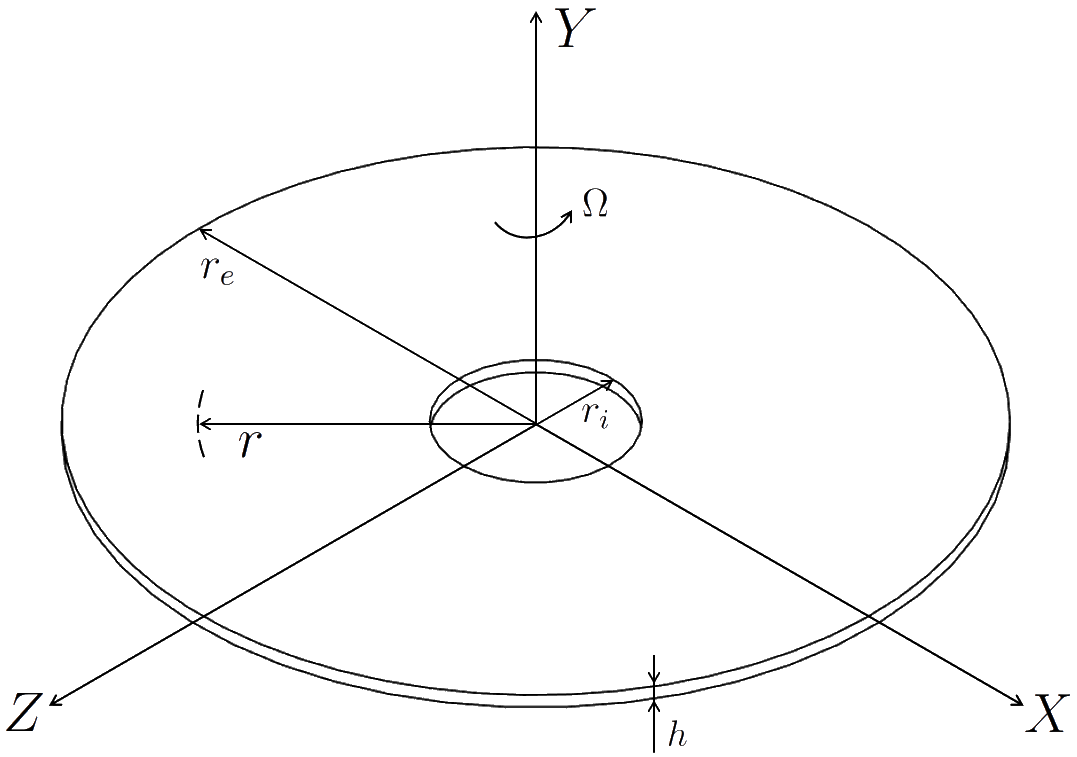
\includegraphics[scale=0.5]{rotating_disk_axisymmetric}
	\caption{Rotating hollow disk.}
	\label{fig:rotating_disk_axisymmetric}
\end{figure}

Theory of elasticity gives the following results for the rotating hollow disk problem. Radial stress, hoop stress, and radial displacement are given in Eqs. ~\ref{equation:sigma_rr}, ~\ref{equation:sigma_tt}, and ~\ref{equation:u_r}, respectively (see Reference \cite{rotors_book}).

\begin{equation}
\label{equation:sigma_rr}
{{\sigma }_{rr}={\frac {(3+{\nu })} {8}}{\rho }{{\omega }^{2}}\left [ {{{r}^{2}_{i}}+{{r}^{2}_{e}}-{{r}^{2}}-{\frac {{{r}^{2}_{i}}{{r}^{2}_{e}}} {{r}^{2}}}} \right ]}
\end{equation}


\begin{equation}
\label{equation:sigma_tt}
{{\sigma }_{{\theta }{\theta }}={\frac {(3+{\nu })} {8}}{\rho }{{\omega }^{2}}\left [ {{{r}^{2}_{i}}+{{r}^{2}_{e}}-\frac {(1+3{\nu })} {(3+{\nu })}{{r}^{2}}+{\frac {{{r}^{2}_{i}}{{r}^{2}_{e}}} {{r}^{2}}}} \right ]}
\end{equation}

\begin{equation}
\label{equation:u_r}
{{u}_{r}={\frac {(3+{\nu })} {8}}{\rho }{{\omega }^{2}}{\frac {(1-{\nu })} {E}r}\left [ {{{r}^{2}_{i}}+{{r}^{2}_{e}}-\frac {(1+{\nu })} {(3+{\nu })}{{r}^{2}}+{\frac {(1+{\nu })} {(1-{\nu })}\frac {{{r}^{2}_{i}}{{r}^{2}_{e}}} {{r}^{2}}}} \right ]}
\end{equation}

\clearpage
\section{Problem Description and Pre-processing}
Problem parameters are given below.\\


Geometry:

$r_i$ $=$ $28$ $mm$,

$r_e$ $=$ $125$ $mm$,

$h$ $=$ $4$ $mm$.\\



Material properties:

$E$ $=$ $2.1 \times 10^{5}$ $MPa$,

$\nu$ $=$ $0.3$,

$\rho$ $=$ $7.8 \times 10^{-9}$  $tonne/mm^{3}$.\\

Loading:

$\Omega$ $=$ $14 \times 10^{3}$ $rpm$.\\

Element type:

$Etyp:$ $qu8cr$.\\

The general purpose quadratic axisymmetric element with reduced integration (CAX8R) is used in CalculiX \cite{CalculiX_website}. One node at $r_i$ is constrained in the axial direction. The finite element model of the rotating hollow disk problem is shown in Figure ~\ref{fig:pre}.

\begin{figure}[h]
	\centering
	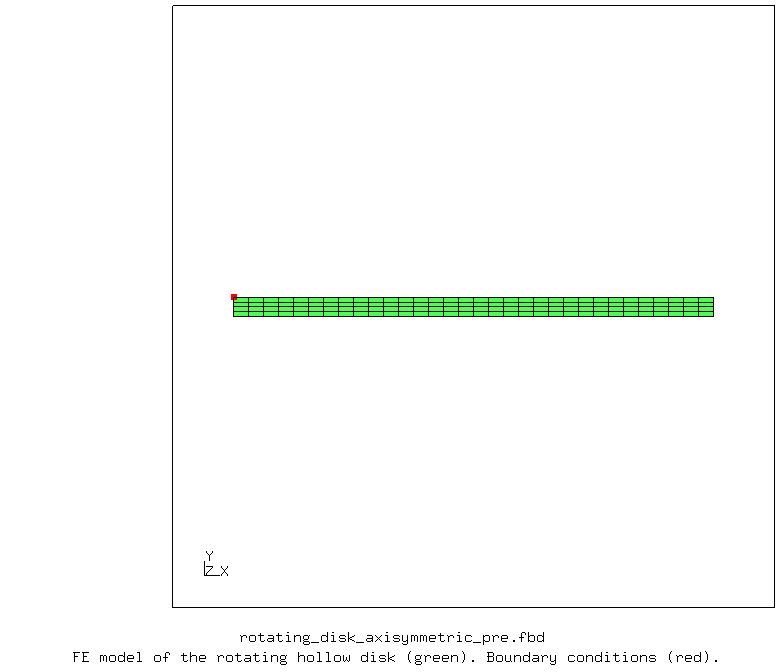
\includegraphics[scale=0.4]{pre}
	\caption{Finite element model of the rotating hollow disk.}
	\label{fig:pre}
\end{figure}

\section{Results}
Dimensionless stresses and displacement are defined below. Comparison between the analytical results obtained from MATLAB and finite element results obtained from CalculiX are presented in Figure ~\ref{fig:rotating_disk_analytical_vs_fe}. Finite element results are extracted from the midline of the 2D axisymmetric disk from $r_i$ to $r_e$.

\begin{equation}
\label{equation:dimensionless_sigma_rr}
{ \overline{{\sigma }}_{rr}=}{\frac {8} {(3+{\nu }){\rho }{{\omega }^{2}{r}^{2}_{e}}}}{\sigma }_{rr}
\end{equation}

\begin{equation}
\label{equation:dimensionless_sigma_tt}
{\overline{\sigma }_{{\theta }{\theta }}=}{\frac {8} {(3+{\nu }){\rho }{{\omega }^{2}{r}^{2}_{e}}}}{\sigma }_{{\theta }{\theta }} 
\end{equation}

\begin{equation}
\label{equation:dimensionless_u_r}
{\overline{u}_{r}=}{\frac {8E} {(3+{\nu })(1-{\nu }){\rho }{{\omega }^{2}{r}^{3}_{e}}}}{u}_{r}
\end{equation}


\textbf{\emph{Analytical Solution}}  \cite{rotors_book}:

Maximum radial stress is 65 MPa.

Minimum radial stress is 0 MPa.

Maximum hoop stress is 218 MPa.

Minimum hoop stress is 57 MPa.

Radial displacement at the inner radius is 0.029119 mm.

Radial displacement at the outer radius is 0.033738 mm.\\


\textbf{\emph{CalculiX Results}}:

Maximum radial stress is 65 MPa.

Minimum radial stress is 0 MPa.

Maximum hoop stress is 218 MPa.

Minimum hoop stress is 57 MPa.


Radial displacement at the inner radius is 0.029116 mm.

Radial displacement at the outer radius is 0.033731 mm.\\

The radial stress, hoop stress, and radial displacements from CalculiX is presented in Figures ~\ref{fig:graph_0}, ~\ref{fig:graph_1}, and ~\ref{fig:graph_2}.


\begin{landscape}
\begin{figure}[h]
	\centering
	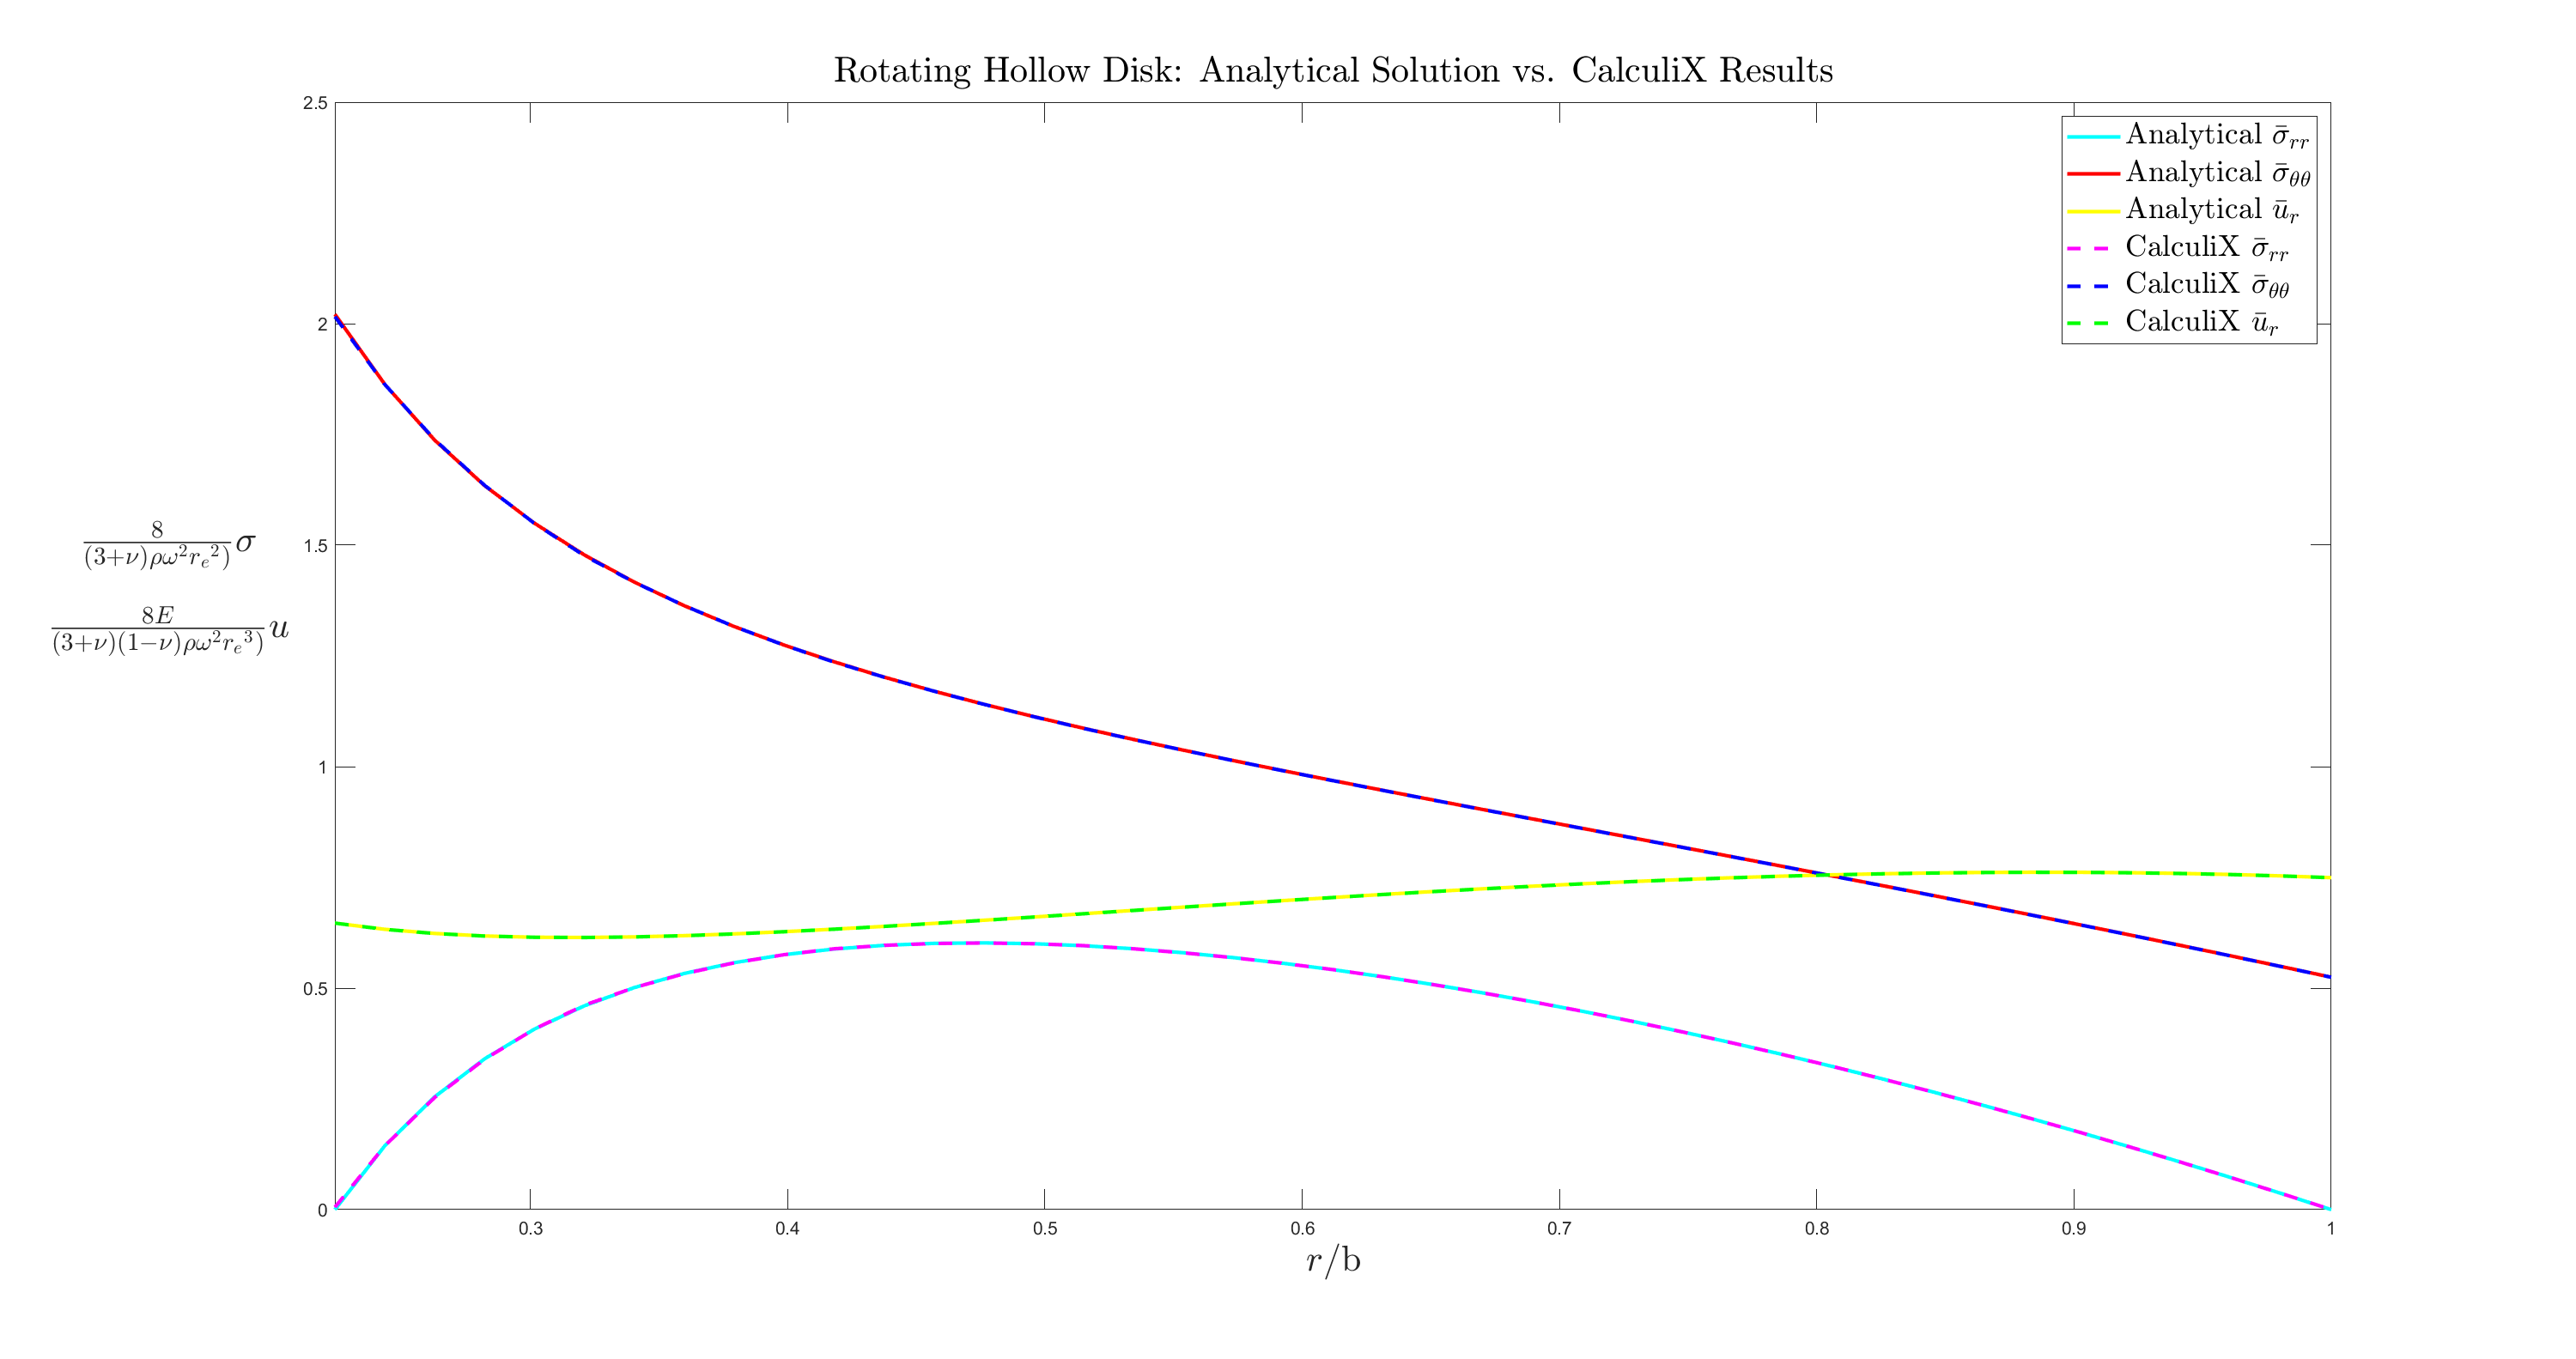
\includegraphics[scale=0.5]{rotating_disk_analytical_vs_fe}
	\caption{Rotating hollow disk: Analytical solution vs. CalculiX results.}
	\label{fig:rotating_disk_analytical_vs_fe}
\end{figure}
\end{landscape}


\begin{figure}[h]
	\centering
	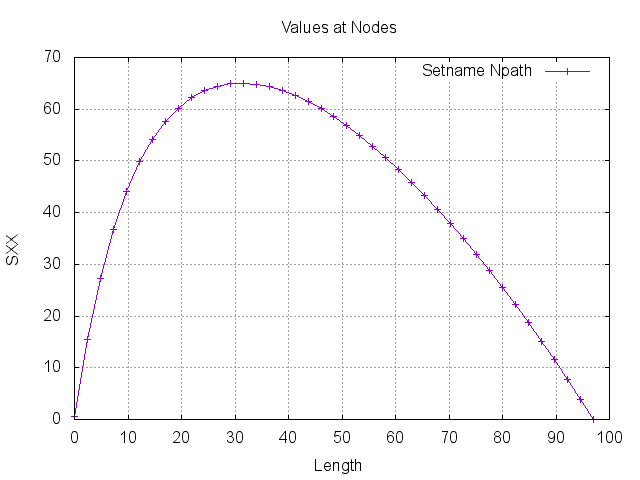
\includegraphics[scale=0.5]{graph_0}
	\caption{CalculiX radial stress plot.}
	\label{fig:graph_0}
\end{figure}

\begin{figure}[h]
	\centering
	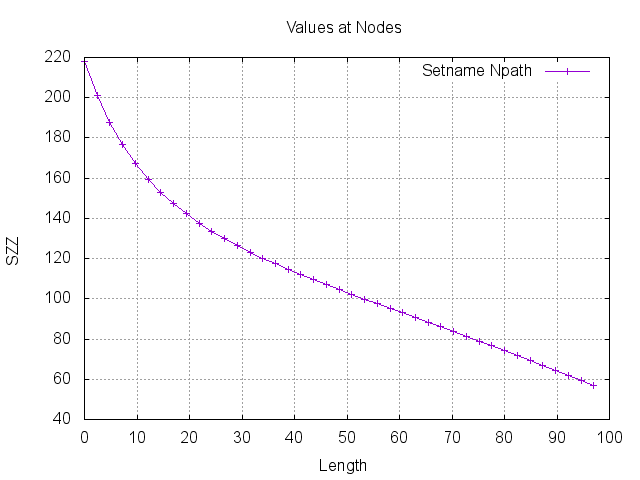
\includegraphics[scale=0.5]{graph_1}
	\caption{CalculiX hoop stress plot.}
	\label{fig:graph_1}
\end{figure}

\begin{figure}[h]
	\centering
	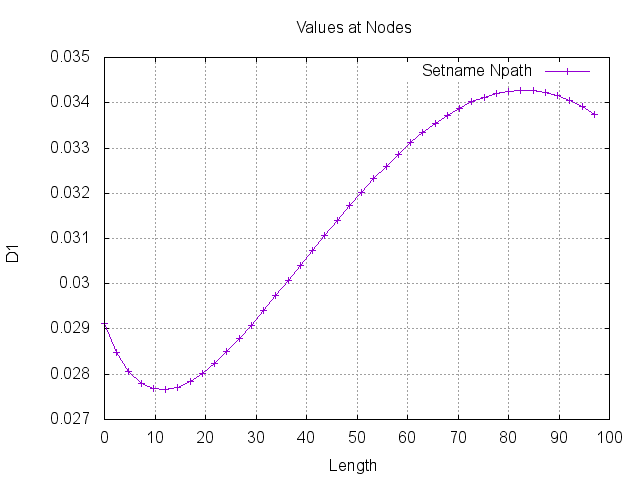
\includegraphics[scale=0.5]{graph_2}
	\caption{CalculiX radial displacement plot.}
	\label{fig:graph_2}
\end{figure}

\clearpage
% Bibliographic references
\begin{thebibliography}{9}
	
\bibitem{CalculiX_website} 
CalculiX, A Free Software Three-Dimensional Structural Finite Element Program. \url{http://www.calculix.de/}

\bibitem{rotors_book} 
Rotors: Stress Analysis and Design, 2013. Page 29, Example 1. 

\end{thebibliography}


\end{document}